\documentclass{report}
\usepackage[utf8]{inputenc}

\title{
    Buildy \\
    \large Applicazioni e Servizi Web
}

\author{Filippo Cavallari - 0001025884 \{filippo.cavallari2@studio.unibo.it\}}
\date{28/05/2022}

\usepackage{natbib}
\usepackage{graphicx}
\usepackage{listings}
\usepackage{color}

\definecolor{dkgreen}{rgb}{0,0.6,0}
\definecolor{gray}{rgb}{0.5,0.5,0.5}
\definecolor{mauve}{rgb}{0.58,0,0.82}

\lstdefinelanguage{JavaScript}{
  keywords={typeof, new, true, false, catch, function, return, null, catch, switch, var, let, const, if, in, while, do, else, case, break},
  keywordstyle=\color{dkgreen}\bfseries,
  ndkeywords={class, export, boolean, throw, implements, import, this, async, await},
  ndkeywordstyle=\color{mauve}\bfseries,
  identifierstyle=\color{black},
  sensitive=false,
  comment=[l]{//},
  morecomment=[s]{/*}{*/},
  commentstyle=\color{purple}\ttfamily,
  stringstyle=\color{red}\ttfamily,
  morestring=[b]',
  morestring=[b]"
}

\lstset{frame=tb,
  language=JavaScript,
  aboveskip=3mm,
  belowskip=3mm,
  showstringspaces=false,
  columns=flexible,
  basicstyle={\small\ttfamily},
  numbers=none,
  numberstyle=\tiny\color{gray},
  keywordstyle=\color{blue},
  commentstyle=\color{dkgreen},
  stringstyle=\color{mauve},
  breaklines=true,
  breakatwhitespace=true,
  tabsize=3
}


\begin{document}

\maketitle
\section{Introduzione}
Buildy è una semplice piattaforma di continuos deployment, facile ad usare ma allo stesso tempo molto potente, per \textit{"buildare"} e \textit{"deployare"} progetti Java basati su Gradle.

\section{Requisiti}
\subsection{Requisiti utente}
L'utente finale di Buildy è un Java Software Engineer o un Java Software Developer che si aspetta di poter:
\begin{itemize}
\item vedere la lista di tutti i progetti registrati con relativo status dell'ultima compilazione
\item poter aggiungere un nuovo progetto
\item poter consultare tutte le compilazioni di un progetto, sia attuali che passate
\item poter accedere ai log di una specifica compilazione
\item poter accedere agli artefatti (.jar) di una specifica compilazione
\item poter ottenere un link ad un badge che si aggiorna in automatico in base allo status dell'ultima compilazione
\end{itemize}

\subsection{Requisiti funzionali}
\begin{itemize}
\item Autenticazione di un utente
\item Registrazione di un nuovo utente
\item Aggiunta di un progetto
\item Monitoraggio costante dei progetti
\item Compilazione dei progetti
\item Pubblicazione dei log delle compilazioni
\item Pubblicazione degli artefatti delle compilazioni
\item Creazione dei badge .SVG per ogni compilazione
\item Cronologia delle compilazioni passate di ogni progetto
\end{itemize}

\subsection{Requisiti non funzionali}
\begin{itemize}
\item Rendere il sistema reattivo (e.g. caricamenti minimi o assenti)
\item Interfaccia utente adatta anche a persone con problemi di visibilità (e.g. daltonismo e cecità)
\item Rendere il processo di autenticazione sicuro
\item Rendere il sistema scalabile in base al carico di lavoro (i.e. compatibilità con docker swarm)
\end{itemize}


\section{Design}
Design dell'architettura del sistema e delle interfacce utente.
\subsection{Interfacce utente}
\begin{figure}[h!]
\centering
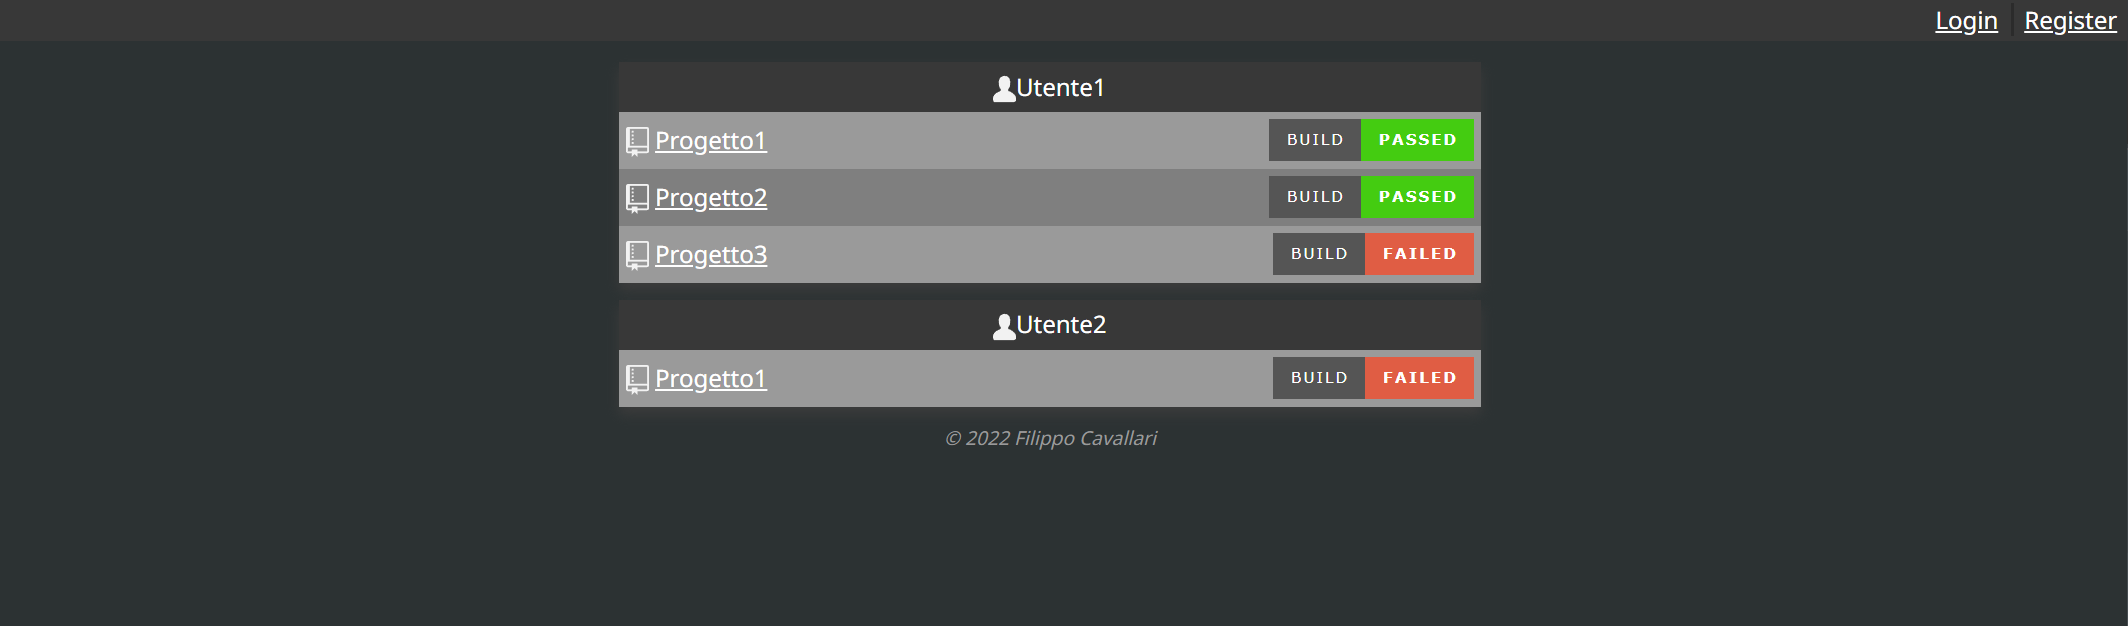
\includegraphics[scale=0.44]{homepage.png}
\caption{Home page}
\label{fig:homepage}
\end{figure}
L'homepage di Buildy (figura \ref{fig:homepage}) contiene la lista di tutti i progetti registrati, raggruppati in base al creatore della repository di ciascun progetto; nella navbar sono inoltre presenti due bottoni per aprire i pannelli per l'accesso e la registrazione.\\
\begin{figure}[h!]
\centering
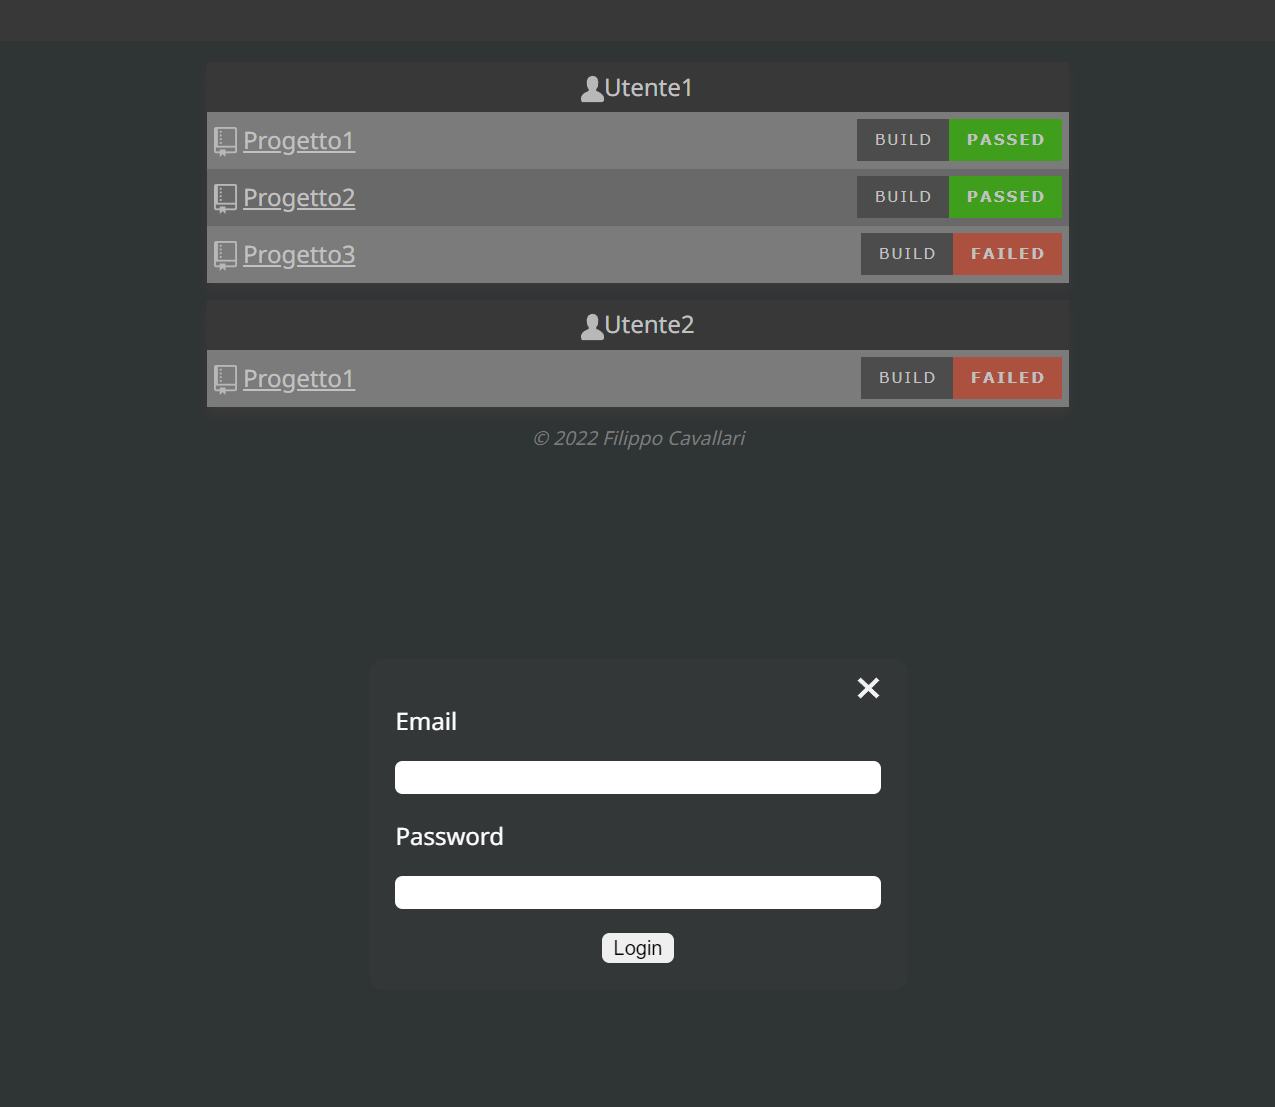
\includegraphics[scale=0.44]{login.png}
\caption{Login modal}
\label{fig:loginmodal}
\end{figure}
Nel pannello di accesso (figura \ref{fig:loginmodal}) vengono richiesti email e password.\\
\begin{figure}[h!]
\centering
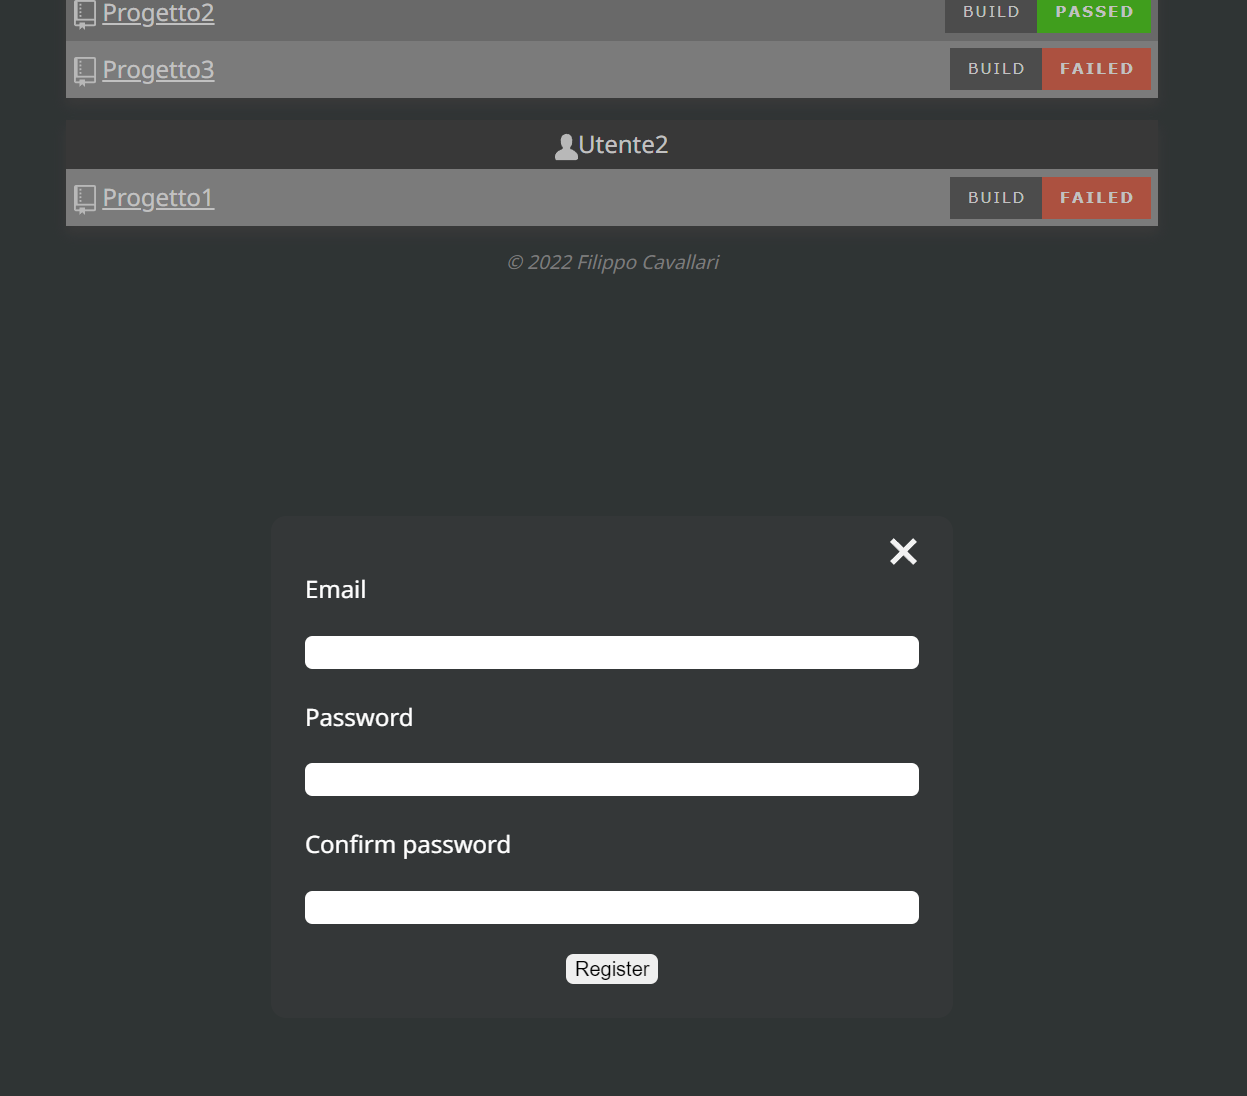
\includegraphics[scale=0.44]{register.png}
\caption{Register modal}
\label{fig:registermodal}
\end{figure}
Nel pannello di registrazione (figura  \ref{fig:registermodal}) vengono chiesti l'email e due volte la password (per evitare errori di scrittura).\\
\begin{figure}[h!]
\centering
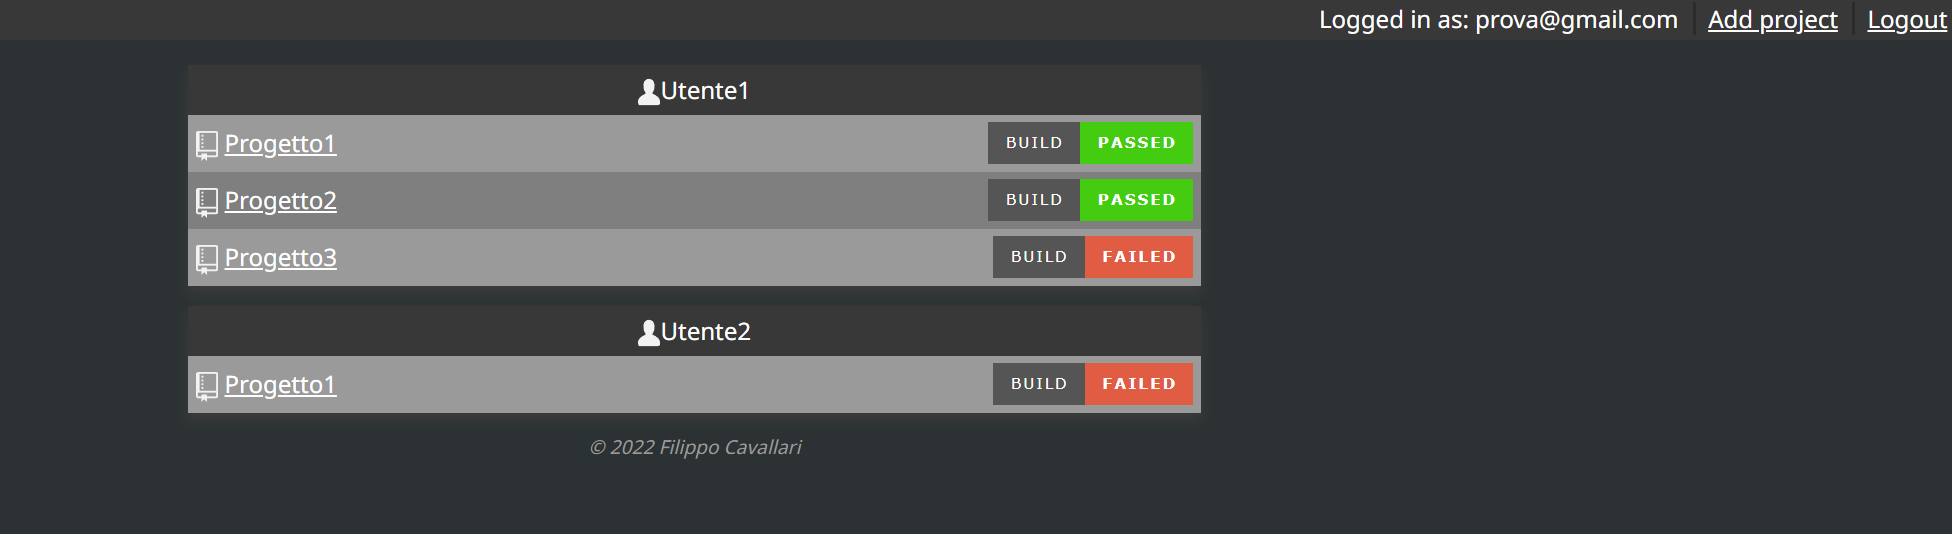
\includegraphics[scale=0.44]{postlogin.png}
\caption{Post authentication home page}
\label{fig:postauthhomepage}
\end{figure}
Dopo aver effettuato l'autenticazione, la home apparirà come in figura \ref{fig:postauthhomepage} ; la navbar mostrerà l'email con la quale si è effettuato l'accesso, un bottone per l'aggiunta di un nuovo progetto ed il bottone per effettuare il logout.\\
\begin{figure}[h!]
\centering
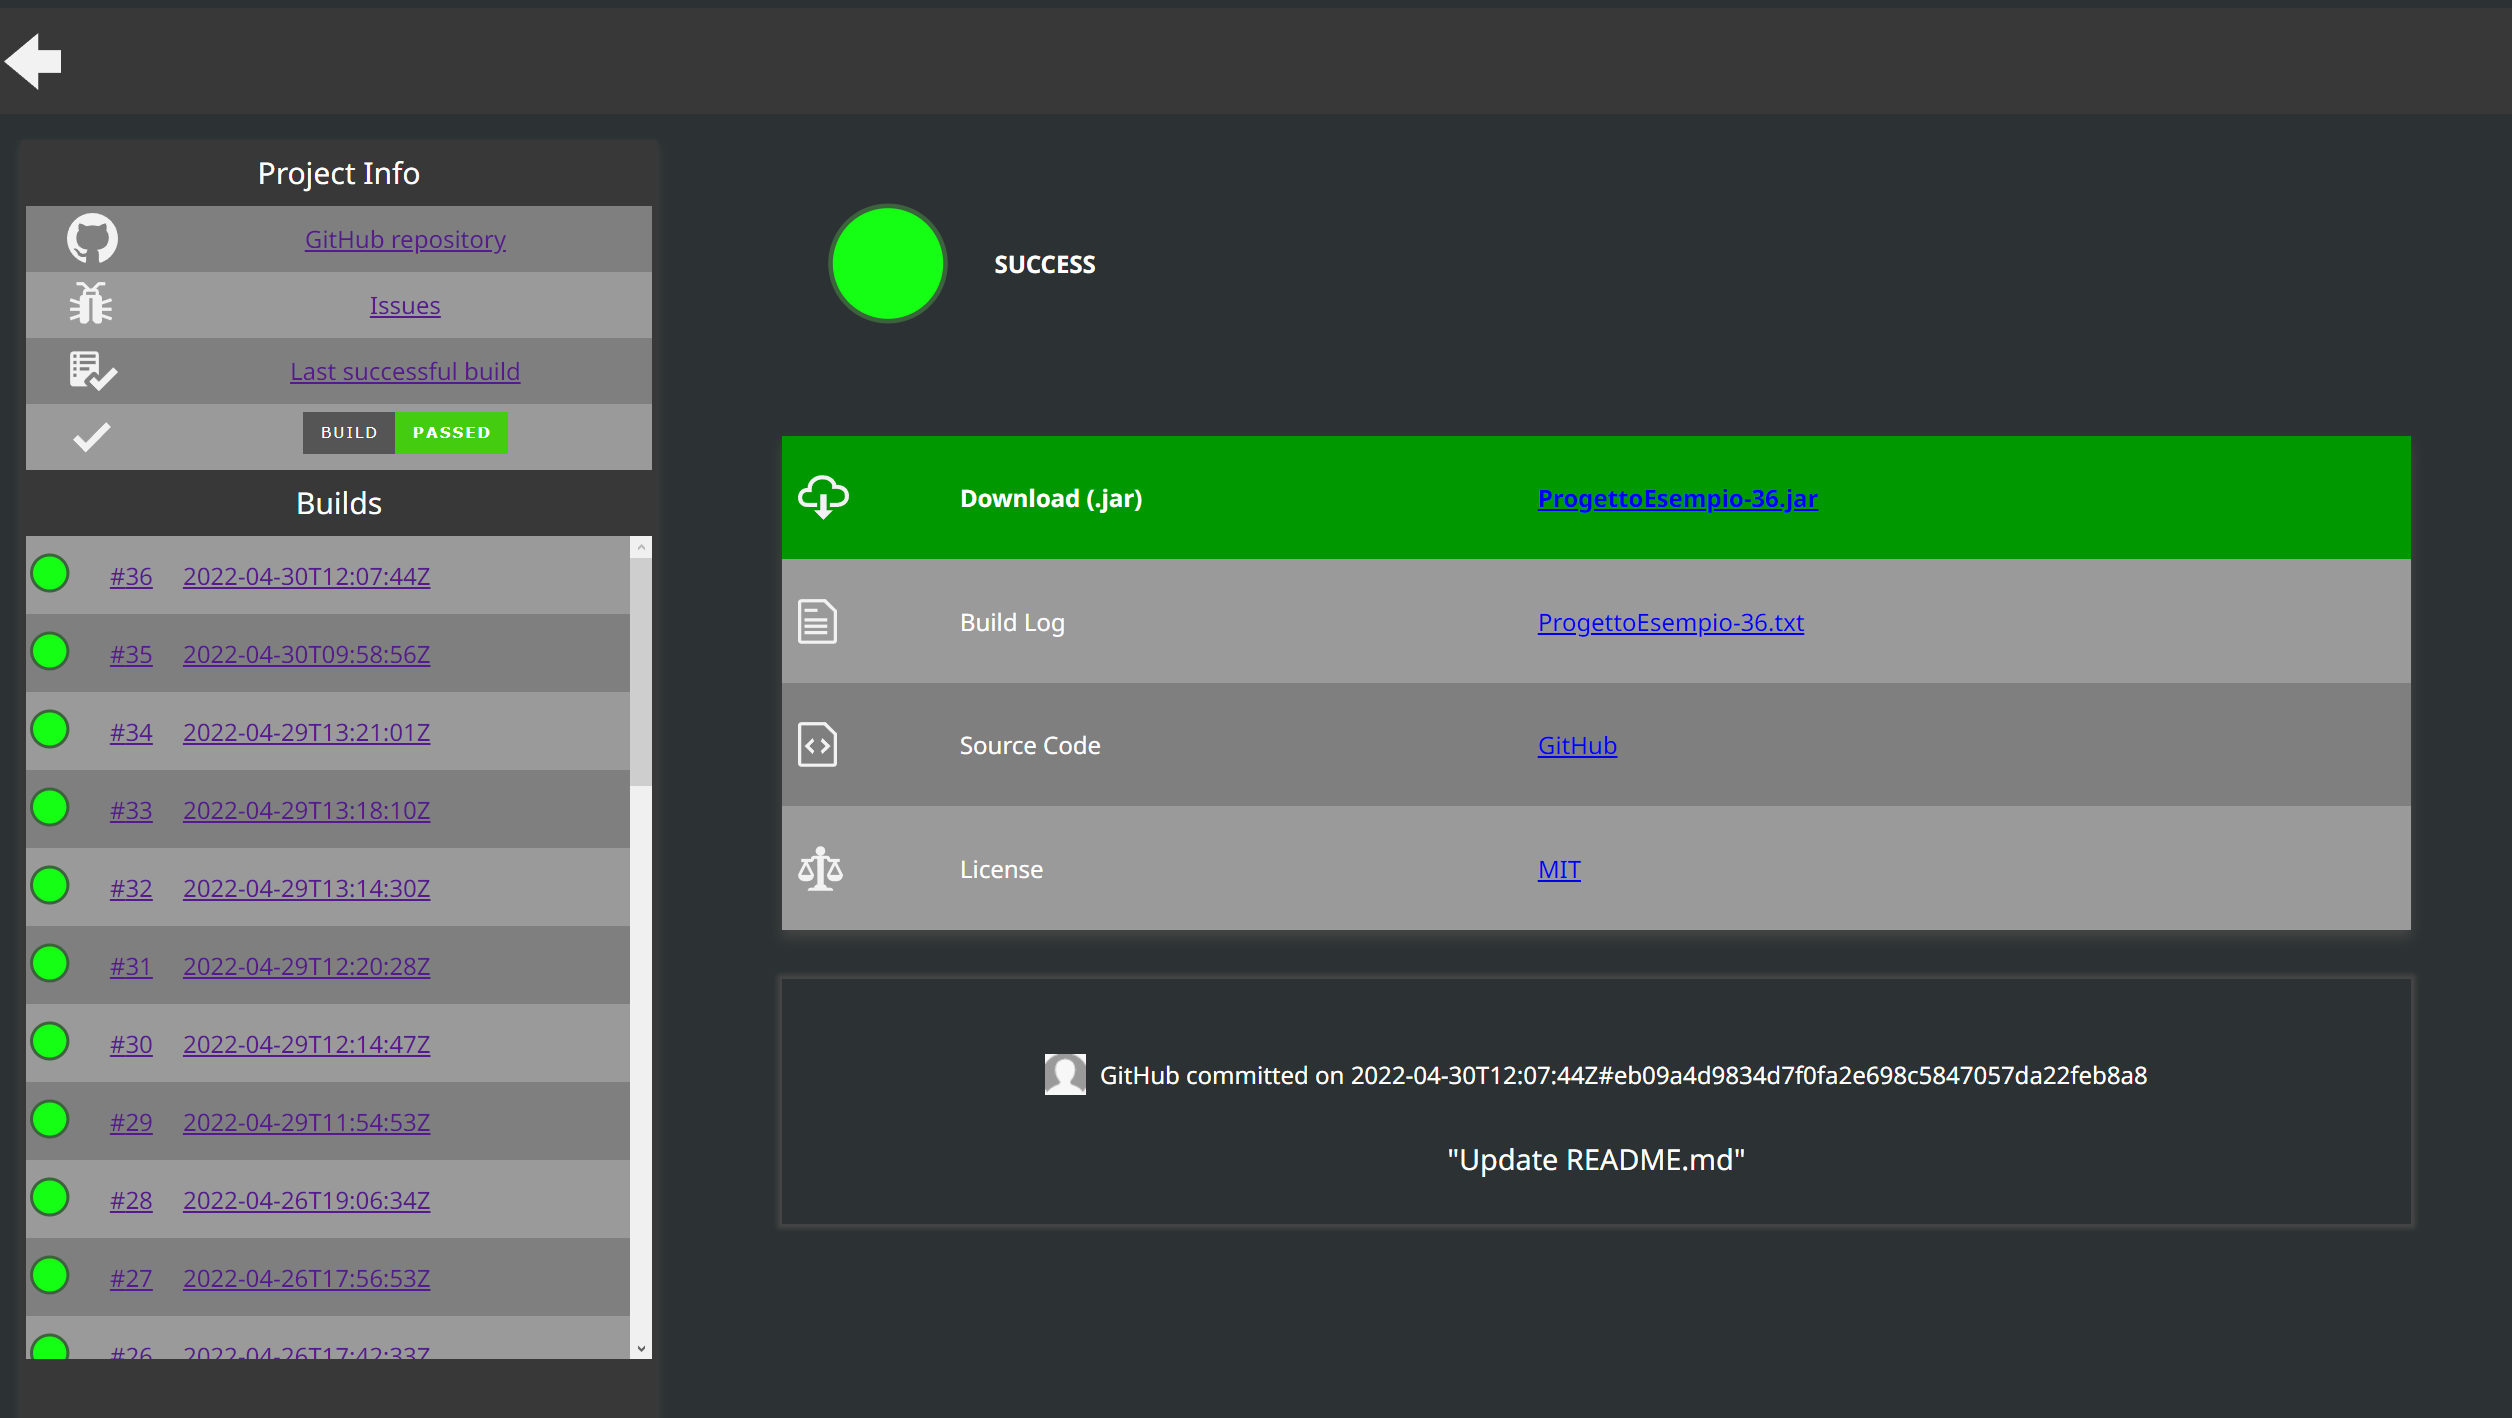
\includegraphics[scale=0.44]{progetto.png}
\caption{Project page}
\label{fig:projectpage}
\end{figure}
Quando si accede alla pagina di un progetto (figura  \ref{fig:projectpage} , si possono: consultare tutte le build passate nella sidebar a sinistra, con tanto di esito, ID e data di compilazione; accedere ai log o agli artefatti cliccando sui relativi link; copiare il link del badge facendo tasto destro $\rightarrow$ copia link dell'immagine; consultare altre informazioni fra cui chi ha effettuato l'ultimo commit, in quale data e con quale messaggio.\\
\begin{figure}[h!]
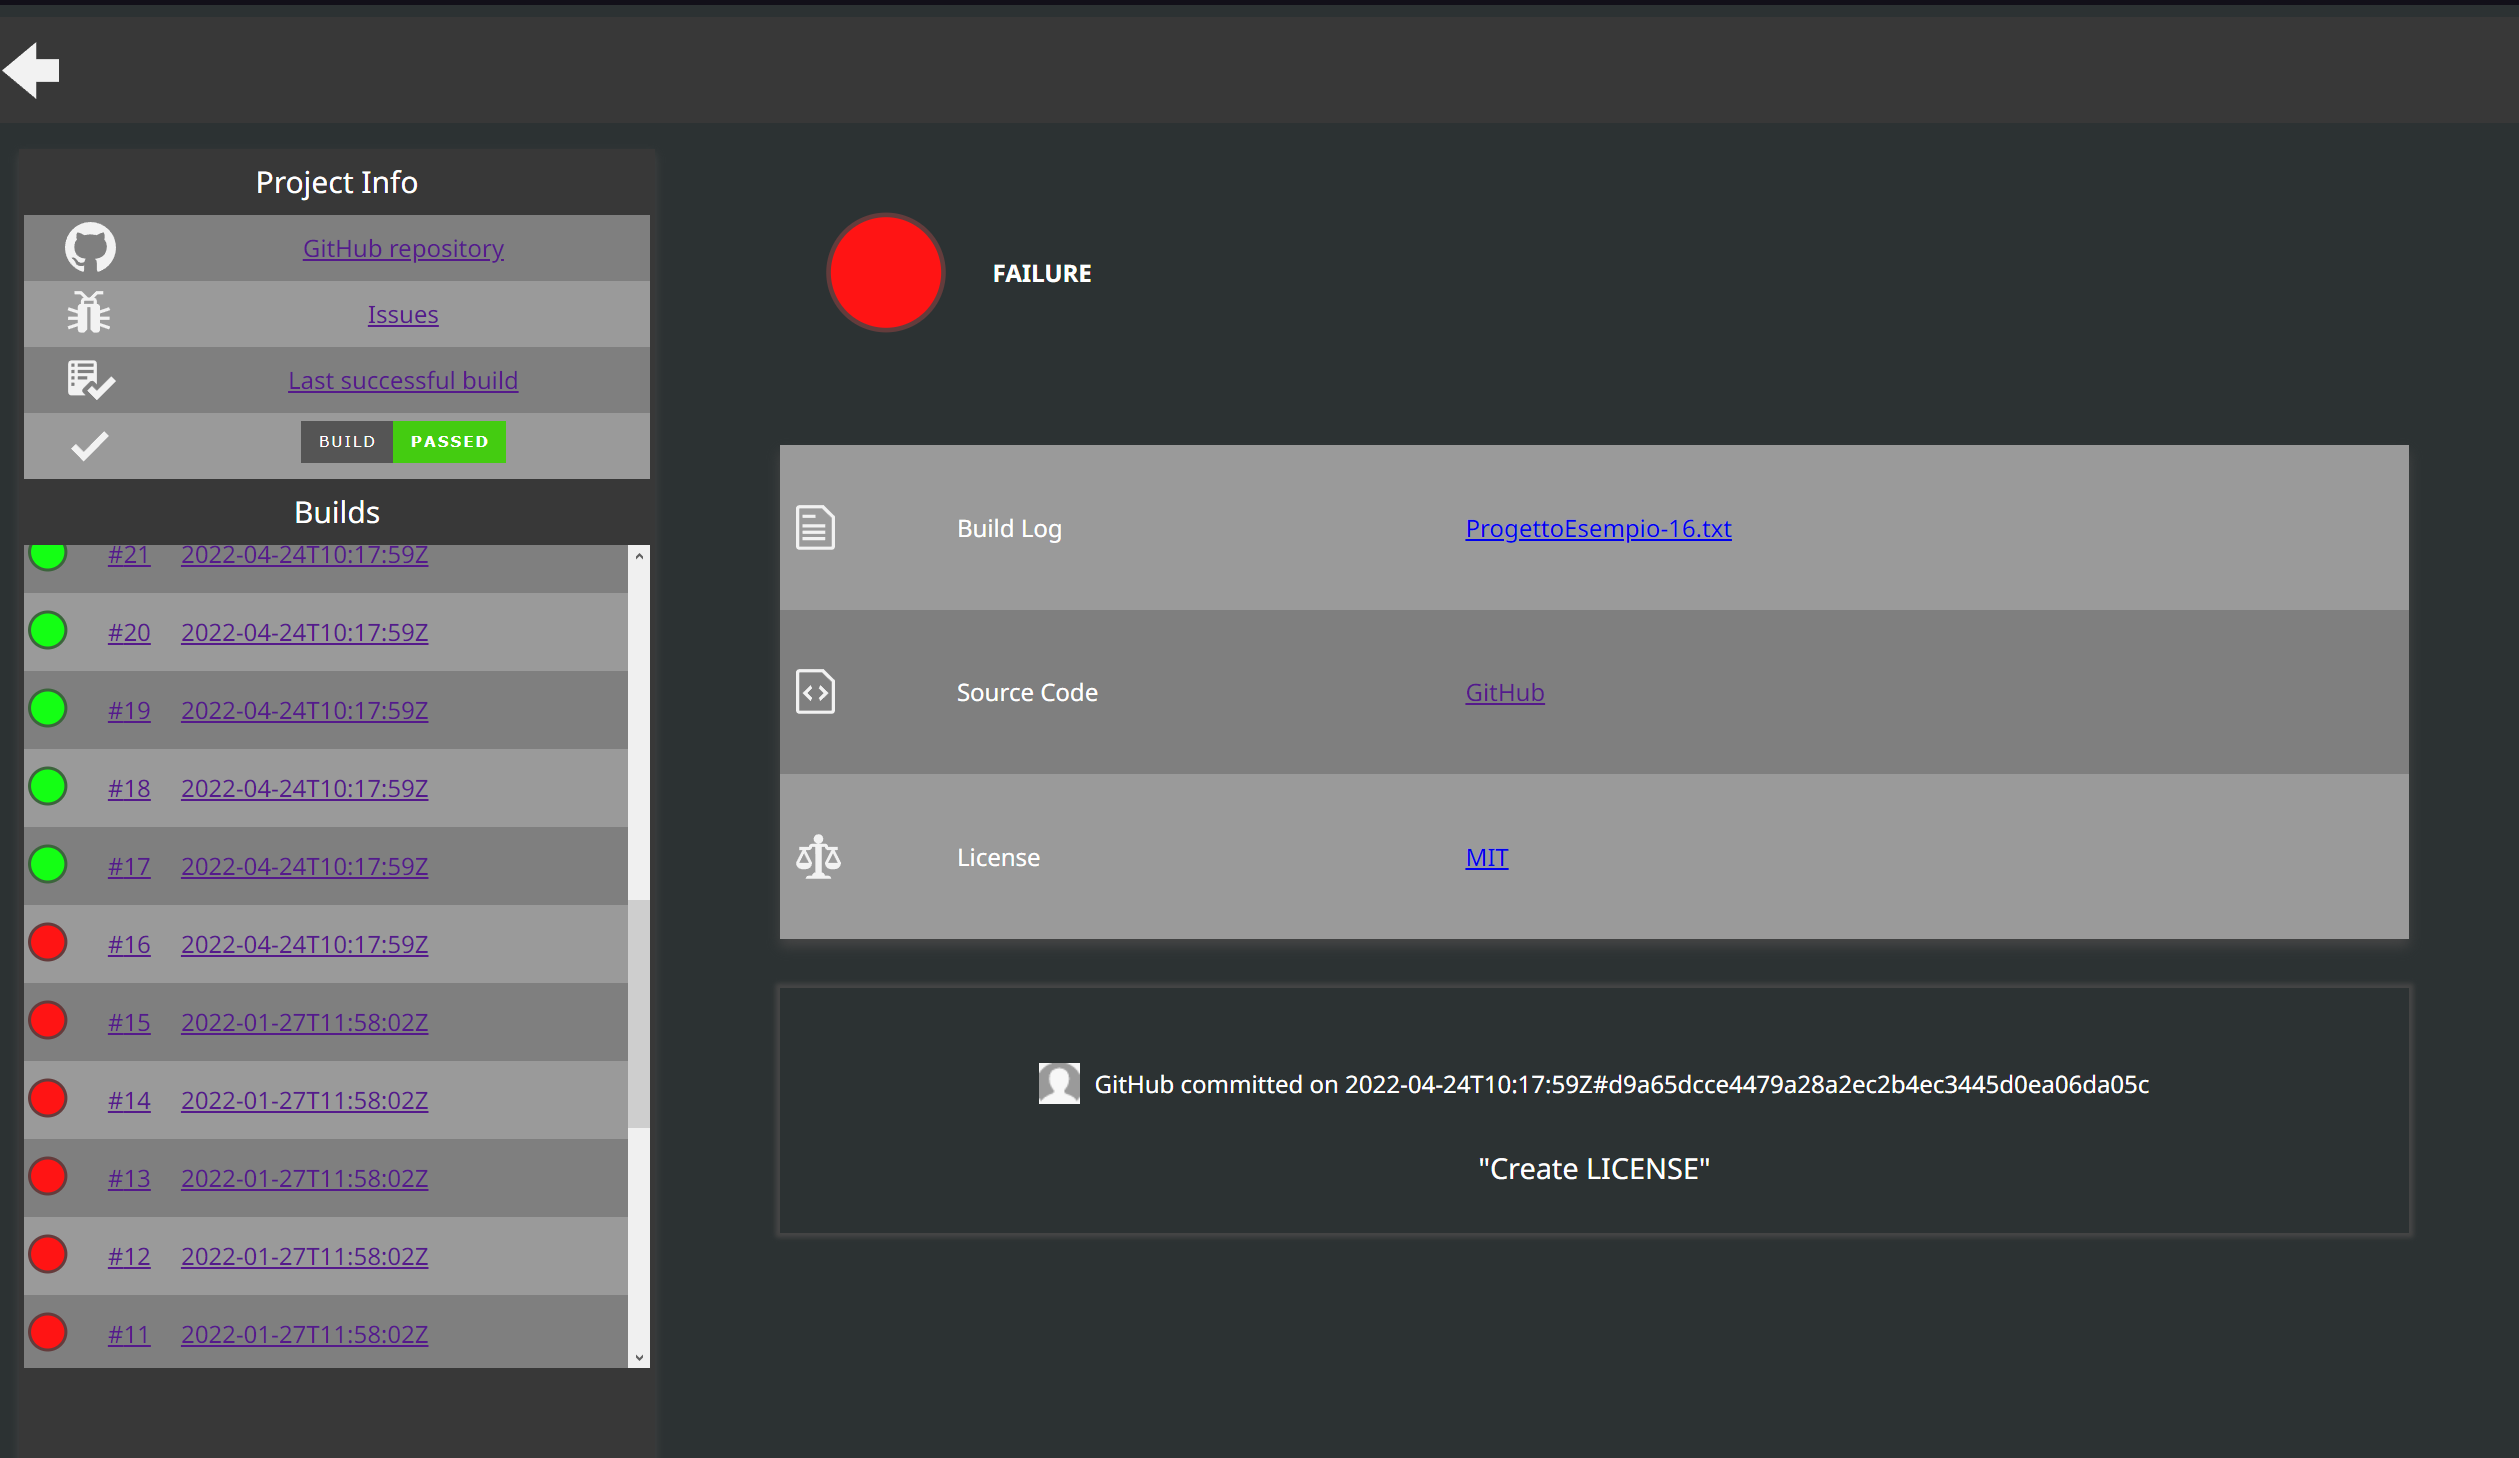
\includegraphics[scale=0.3]{progetto fail.png}
\caption{Failed build project page}
\label{fig:projectfail}
\end{figure}
Quando una build fallisce (figura \ref{fig:projectfail}) non sarà possibile accedere agli artefatti (se non compila non potrà aver prodotto artefatti), il colore dello status diventerà rosso e se si tratta dell'ultima compilazione allora anche il badge verrà aggiornato di conseguenza (colore rosso ed etichetta "FAILED").
\subsection{Architettura del sistema}
\subsubsection{Frontend}
Il frontend è realizzato con React; si occupa di renderizzare l'applicazione e gestire l'input dell'utente. Tutte le richieste HTTP vengono realizzate usando il modulo axios mentre per lo scambio di dati reattivo e con basso overhead viene usato socket.io. \\
I fogli di stile sono stati realizzati con Sass e poi compilati in automatico dall'IDE in modo da avere dei file CSS3 tradizionali.\\
È stata data molta importanza all'usabilità da parte di persone con problemi di vista, sia parzialmente che totalmente invalidanti; per esempio per le persone daltoniche che non riescono a distiguere il verde dal rosso, è stata scritto l'esito della build all'interno del badge (SUCCESS o FAILURE); anche la scelta di usare un font chiaro su sfondo scuro permette una maggiore leggibilità; inoltre tutte le immagini hanno un tag \textit{alt} in modo che siano compatibili con lettori di testo usati da persone non vedenti.

\subsubsection{Backend}
Il backend è realizzato usando NodeJS+Express;  si occupa essenzialmente di gestire il processo di compilazione dei processi e di scambiare dati con il frontend (React) attraverso gli endpoint di Express e il websocket di socket.io.\\
Andando più nel dettaglio si possono distinguere tre funzionalità chiave.

\textbf{Compilazione progetti:}
\begin{enumerate}
\item Ogni 10 minuti controlla ogni progetto per vedere se sono stati effettuati nuovi commit;
\item Se ci sono nuovi commit clona il progetto e lo compila;
\item Gli artefatti, i file di log e il badge .SVG vengono pushati su GitHub
\item Vengono aggiornate le informazioni del progetto (e.g. last build, last commit) sul DB
\end{enumerate}
\textbf{Autenticazione utente:}
\begin{enumerate}
\item Le credenziali dell'utente vengono ricevute da una richiesta HTTP POST (usando il modulo \textit{axios}) in modo che i data vengano cifrati usando il TLS;
\item Le password non sono salvate in chiaro sul DB, ma vengono cifrate usando una funzione di hash (sha512) con l'aggiunta di un sale;
\item se le credenziali fornite sono corrette, l'utente viene autenticato e viene emesso un nuovo token di autenticazionel;
\item tale token verrà inserito in un cookie \textit{HTTP only} (per motivi di sicurezza) e scadrà dopo sette giorni;
\item per ogni richiesta HTTP verrà controllato il token di autenticazione presente nel cookie e, in caso di responso positivo, la richiesta dell'utente verrà soddisfatta. 
\end{enumerate}
\textbf{Richiesta dati dal frontend:}
\begin{enumerate}
\item Tutte le richieste di dati che non necessitano di autenticazione vengono effettuate usando socket.io;
\item Quando l'homepage viene caricata, React richiederà al backend la lista di tutti i progetti con tanto di badge .SVG;
\item Quando un progetto specifico viene aperto, React richiederà la cronologia di tutte le compilazioni più altre informazioni.
\end{enumerate}

\subsubsection{Docker}
Tutti i componenti di Buildy sono stati dockerizzati in modo che possono essere eseguiti facilmente usando i comandi di docker-compose.
\section{Tecnologie}
Si è utilizzato come solution stack MERN.
Le tecnologie utilizzate per sviluppare il sistema sono:
\begin{itemize}
\item  Node ed Express: sviluppo componente server;
\item React : sviluppo componente client;
\item MongoDB: gestione persistenza dati;
\item Socket.io: scambio dati real time;
\item Docker: per il deploy dell’applicazione.
I linguaggi utilizzati all’interno del progetto sono:
\item Javascript (ES6): sia lato client che lato server;
\item JSX: per la struttura delle pagine web;
\item Scss: per i fogli di stile;
\end{itemize}

\section{Codice}
\begin{lstlisting}
async function main(){
    projects = await getProjectsFromDb()
    await setGitIdentity()
    for (const project of projects) {
        await analyzeProject(project)
    }
    console.log("Saving projects on db")
    await saveProjectArray(projects)
}

async function analyzeProject(project){
    console.log(`Retrieving last commit for project ${project.projectName}`)
    let latestCommit = await getLatestCommit(project)
    let sha = latestCommit.sha
    console.log(`Retrieving repository data for project ${project.projectName}`)
    await project.repository.getInformation()
    if(sha !== project.latestCommitSha){
        console.log(`Cloning  project ${project.projectName}`)
        await project.clone()
        console.log(`Building project ${project.projectName}`)
        let build = await project.build(latestCommit)
        console.log(`Saving build ${build.id} for project ${project.projectName}`)
        await project.saveBuild(build)
        console.log(`Pushing build ${build.id} for project ${project.projectName}`)
        await project.commitBuild(build)
    }
}
\end{lstlisting}
Le funzioni main() e analyzeProject(), entrambe asincrone, sono il fulcro del backend; la funzione main viene invocata ogni 10 minuti e si occupa di invocare la funzione \textit{analyzeProject} su ciascun progetto registrato per poi aggiornarli nel DB; la funzione \textit{analizeProject} è invece quella che effettua l'analisi vera e propria del progetto; l'analisi si suddivide nei seguenti step:
\begin{enumerate}
\item \textit{getLatestCommit()}: recuperare lo SHA dell'ultimo commit
\item \textit{repository.getInformation()}: recupera le informazioni sulla repository del progetto (e.g. commit messagge, commit timestamp, clone url, ecc.)
\item verifica che lo SHA dell'ultimo commit sia diverso da quello dell'ultima compilazione effettuata
\item \textit{project.clone()}: clona il progetto
\item \textit{project.build()}: compila il progetto
\item \textit{project.saveBuild()}: serve a serializzare la classe Build; in altre parole crea il badge .SVG, crea i file di log e sposta gli artefatti nella destinazione finale
\item \textit{project.commitBuild()}: carica gli artefatti e i log su GitHub
\end{enumerate}
Tutte le funzioni sono asincrone.


\begin{lstlisting}
function registerListeners(socketIO){
    socketIO.on('connection', (socket) => {
        socket.on('project-page-request', (message) => {
            let proj = getProjects().filter(it => it.projectName === message.projectName)[0]
            socketIO.emit('project-page-response', {project: proj, builds: [...proj.builds].reverse(), latestBuildId: proj.builds.slice(-1)[0].id})
        })
        socket.on('index-page-request', ()=>{
            let authors = []
            let projects = getProjects()
            for(const proj of projects){
                let authorName = proj.repository.owner
                let filterResult = authors.filter((author) => author.name === authorName)[0]
                if(filterResult === undefined){
                    let author = {name: authorName, projects: [proj]}
                    authors.push(author)
                }else{
                    filterResult.projects.push(proj)
                }
            }
            socketIO.emit('index-page-response', {authors: authors})
        })
    });
}
\end{lstlisting}
La funzione \textit{registerListeners()} si occupa di registrare i listener di \textit{socket.io}; nello specifico vengono creati due listener, uno per le richieste dei dati della homepage (\textit{index-page-request}), ed uno per le richieste dei dati di un progetto specifico (\textit{project-page-request}).\\
Quando il websocket riceve una richiesta la elabora ed emette un nuovo evento (i.e. \textit{index-page-response} o \textit{project-page-response}) con i dati richiesti.
\begin{lstlisting}
function cloneProject(project){
    return spawn("git", ["clone", "-b", project.mainBranch, project.repository.cloneUrl, `projects/${project.repository.name}`], { stdio: 'inherit' })
}
\end{lstlisting}
La funzione cloneProject() crea un processo figlio al quale fa clonare il progetto che viene passato negli argomenti del comando git; lo stdin e lo stdout vengono ereditati dal processo padre, di conseguenza i log verranno scritti negli stream (di default il terminale) di NodeJs.
\begin{lstlisting}
async build(latestCommit) {
        await fs.promises.chmod(`projects/${this.repository.name}/gradlew`, 0o777)
        let gradleBuildScript = path.resolve(`src/gradle_build.sh`)
        return new Promise((resolve, reject) => {
            let log = ""
            let child = child_process('bash', [gradleBuildScript, this.repository.name], {shell: true})
            child.stdout.on('data', (data) => log += data)
            child.stderr.on('data', (data) => log += data);
            child.on('close', (code) => {
                if (code === 0) {
                    resolve(this.createBuild(latestCommit, true, log))
                } else {
                    resolve(this.createBuild(latestCommit, false, log))
                }
            });
        })
    }
\end{lstlisting}
La funzione \textit{build()} si occupa di compilare un progetto; per poterlo fare aggiunge i permessi di esecuzione ad un apposito script bash e poi lo fa eseguire ad un processo figlio; quest'ultimo avrà gli stdin e stdout indipendenti, i cui dati verranno incanalati all'interno di una variabile \textit{log} che verrà poi passata come argomento del costruttore della classe \textit{Build} per un successivo utilizzo.
\begin{lstlisting}
async saveBuild(build) {
        this.latestCommitSha = build.commitSha
        this.wasModified = true
        build.logFileName = `${this.projectName}-${build.id}.txt`
        this.builds.push(build)
        await fs.promises.mkdir(`builds/${this.projectName}/`, {recursive: true})
        if (build.isSuccess) {
            console.log(this.projectName)
            let buildFolder = `projects/${this.repository.name}/build/libs/`
            let buildFile = (await fs.promises.readdir(buildFolder)).filter((allFilesPaths) =>
                allFilesPaths.match(/\.jar$/) !== null)[0]
            let buildPath = buildFolder + buildFile
            let splintedBuildFileName = buildFile.split(".")
            build.fileName = `${splintedBuildFileName[0]}-${build.id}.${splintedBuildFileName[1]}`
            await fs.promises.rename(buildPath, `builds/${this.projectName}/${splintedBuildFileName}`)
        }
        await fs.promises.writeFile(`builds/${this.projectName}/${build.logFileName}`, build.log, "utf-8")
        await this.createBadge(build)
        return fs.promises.rm(`projects/`, {recursive: true, force: true})
    }
\end{lstlisting}
La funzione \textit{saveBuild()}, come accennato in precedenza, si occupa di "serializzare" la classe \textit{Build}; occorre quindi che crei i file di log, che sposti gli artefatti dalla cartella di output della compilazione in una nuova destinazione, ed infine creare il badge .SVG (invocando la funzione \textit{createBadge()})
\begin{lstlisting}
 async commitBuild(build) {
        let scriptPath = path.resolve(`src/commit_build.sh`)
        return new Promise((resolve) => {
            let child = child_process("bash", [scriptPath, this.repository.name, build.fileName, build.logFileName, process.env.MYTOKEN], {stdio: 'inherit', env: {...process.env}})
            child.on('close', (code) => {
                if (code === 0) {
                    resolve(true)
                } else {
                    resolve(false)
                }
            })
        })
    }
\end{lstlisting}
La funzione commitBuild() crea un processo figlio e gli fa eseguire uno script bash; quest'ultimo contiene tutti gli step per caricare su GitHub (committare e pushare) i vari file della compilazione; per poter effettuare questa operazioni occorre utilizzare un personal access token che verrà utilizzato da GitHub per autenticare la richiesta.
\begin{lstlisting}
function encryptPassword(password){
    const salt = genRandomString(8)
    return sha512(password, salt)
}

function verifyPassword(passwordHash, password, salt){
    return sha512(password, salt).passwordHash === passwordHash
}

const genRandomString = function (length) {
    return crypto.randomBytes(Math.ceil(length / 2))
        .toString('hex') /** convert to hexadecimal format */
        .slice(0, length);   /** return required number of characters */
};

const sha512 = function(password, salt){
    const hash = crypto.createHmac('sha512', salt); /** Hashing algorithm sha512 */
    hash.update(password);
    const value = hash.digest('hex');
    return {
        salt:salt,
        passwordHash:value
    };
};
\end{lstlisting}
La funzione \textit{encryptPassword()} riceve in input una password in chiaro e restituisce l'output della funzione di hash \textit{sha512} con l'aggiunta di un sale; in questo modo anche in caso di furto dell'hash della password, senza avere accesso al sale sarà impossibile risalire alla password originale.
La funzione \textit{verifyPassword()} controlla che l'hash della password in chiaro con l'aggiunta del sale sia uguale all'hash passato come parametro (normalmente l'hash salvato sul DB).
La funzione \textit{getRandomString()} fornisce una stringa di lunghezza N (dove N è un parametro) da usare per la generazione del sale.
La funzione \textit{sha512() }è la funzione di hash che accetta come parametri la password in chiaro ed il sale.

\section{Test}
\subsection{Postman}
Per testare il corretto funzionamento degli endpoint di Express è stato utilizzato Postman Desktop come mostrato in figura \ref{fig:postman}.
\begin{figure}[h!]
\centering
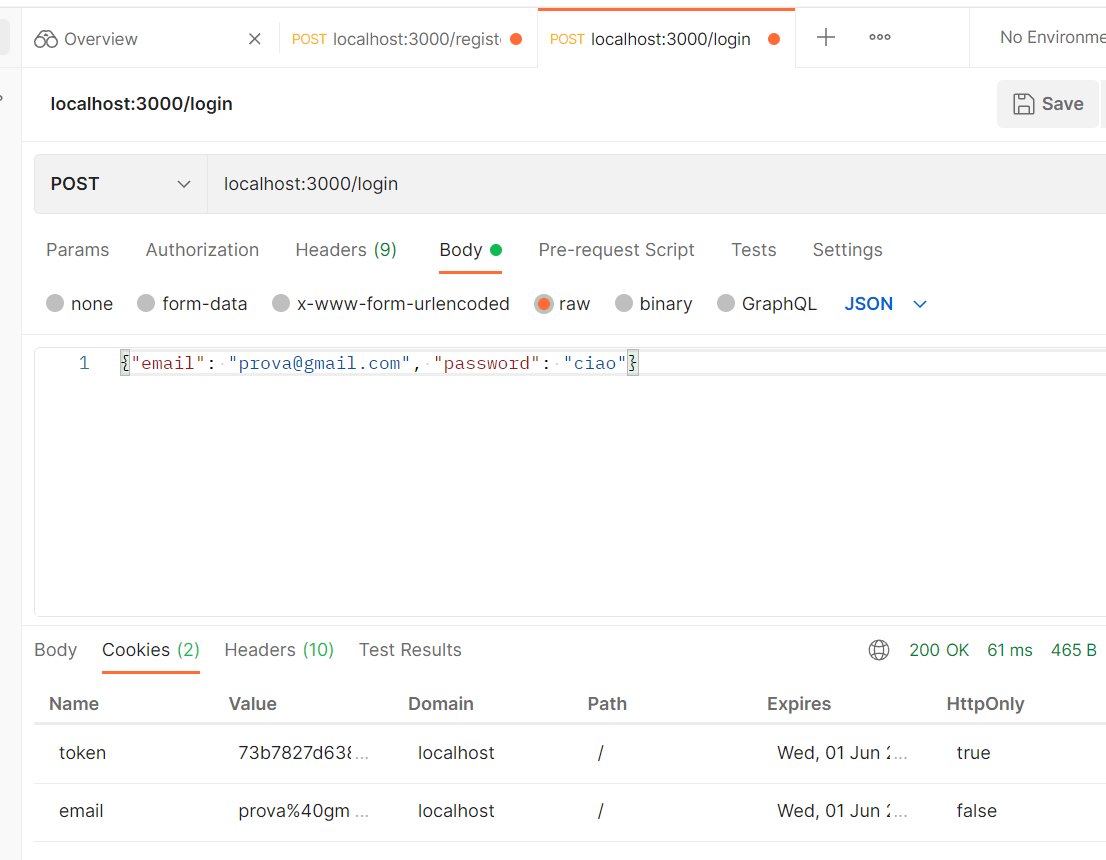
\includegraphics[scale=0.44]{postman.png}
\caption{Postman test}
\label{fig:postman}
\end{figure}
\subsection{Utente}
Buildy è stato testato da altri studenti che hanno aggiunto i propri progetti e sono rimasti molto soddisfatti; in particolare hanno apprezzato:
\begin{itemize}
\item la semplicità d'utilizzo
\item l'assenza di bug
\item il design dell'interfaccia utente
\end{itemize}
I nomi degli studenti non verranno scritti per loro richiesta ma hanno acconsentito ad essere nominati verbalmente.
\section{Deployment}
\textbf{Requisiti:} [\textit{Docker}, \textit{Docker-compose}]
Per installare Buildy è sufficiente clonare la repository ed eseguire il comando \textit{docker-compose up --build -d}.\\
Prima di eseguire il comando è necessario creare un file .env nella root del progetto con le seguenti variabili:
Installare una copia
\lstset{frame=tb,
  language=bash,
  aboveskip=3mm,
  belowskip=3mm,
  showstringspaces=false,
  columns=flexible,
  basicstyle={\small\ttfamily},
  numbers=none,
  numberstyle=\tiny\color{gray},
  keywordstyle=\color{blue},
  commentstyle=\color{dkgreen},
  stringstyle=\color{mauve},
  breaklines=true,
  breakatwhitespace=true,
  tabsize=3
}
\begin{lstlisting}
MYTOKEN=<your_github_personal_access_token>
MONGO_IP=mongodb #You can leave that unchanged, unless you modify the MongoDB container's name
NODE_IP=nodejs #You can leave that unchanged, unless you modify the NodeJS container's name
REACT_IP=localhost #You can leave that unchanged, unless your react container is on a different IP
REPO_URL=github.com/Filocava99/Buildy.git #Set your repository URL (used for storing artifacts and log files)
\end{lstlisting}
Vanno inoltre modificate le variabile in frontend/src/settings.js in modo che combacino con le variabili d'ambiente e le vostre eventuali preferenze.\\
È altamente raccomandato di modificare le credenziali dell'utente root di MongoDB all'interno del file docker-compose.yml per ovvi motivi di sicurezza.\\
Una volta avviato, Buildy sarà raggiungibile sulla porta 80 del vostro dispostivo (http://localhost se l'accesso viene effettuato in locale); il backend utilizza la porta 3000 per Express e la porta 3001 per socket.io.\\
\\
Per testare l'applicazione si consiglia di aggiungere il seguente progetto Gradle:\\
\begin{itemize}
\item ProjectName: Fortress
\item Owner: filocava99
\item Repository: Fortress
\end{itemize}
Dopo aver aggiunto il progetto aspettare che il pannello si chiuda da solo (potrebbero volerci da alcuni secondi ad un minuto, dipende dalla quantità di tempo richiesta per compilare il progetto).


\section{Conclusioni}
Sono personalmente molto soddisfatto da come ho realizzato Buildy; ho in mente diverse modifiche che effettuerò in futuro, fra cui aggiungere il supporto a progetti Maven. Ho anche realizzato una versione basata interamente su NodeJs hostata tramite GitHub pages che può essere facilmente installa forkando la repository.
Spero che possa nascere una piccola community di utilizzatori per entrambi le versioni; proprio per questo ho realizzato un README abbastanza dettagliato e sto lavorando ad una guida su come contribuire ai progetti.
\end{document}
